\documentclass[border=10pt]{standalone}
\usepackage{tikz}
\usepackage{helvet}
\renewcommand{\familydefault}{\sfdefault}
\usetikzlibrary{positioning,arrows.meta,fit,backgrounds}

\definecolor{cData}{HTML}{2C3E50}
\definecolor{cRNA}{HTML}{2980B9}
\definecolor{cAnchor}{HTML}{16A085}
\definecolor{cActivity}{HTML}{8E44AD}
\definecolor{cPheno}{HTML}{D35400}
\definecolor{cNull}{HTML}{C0392B}
\definecolor{cBg}{HTML}{ECF0F1}

\begin{document}
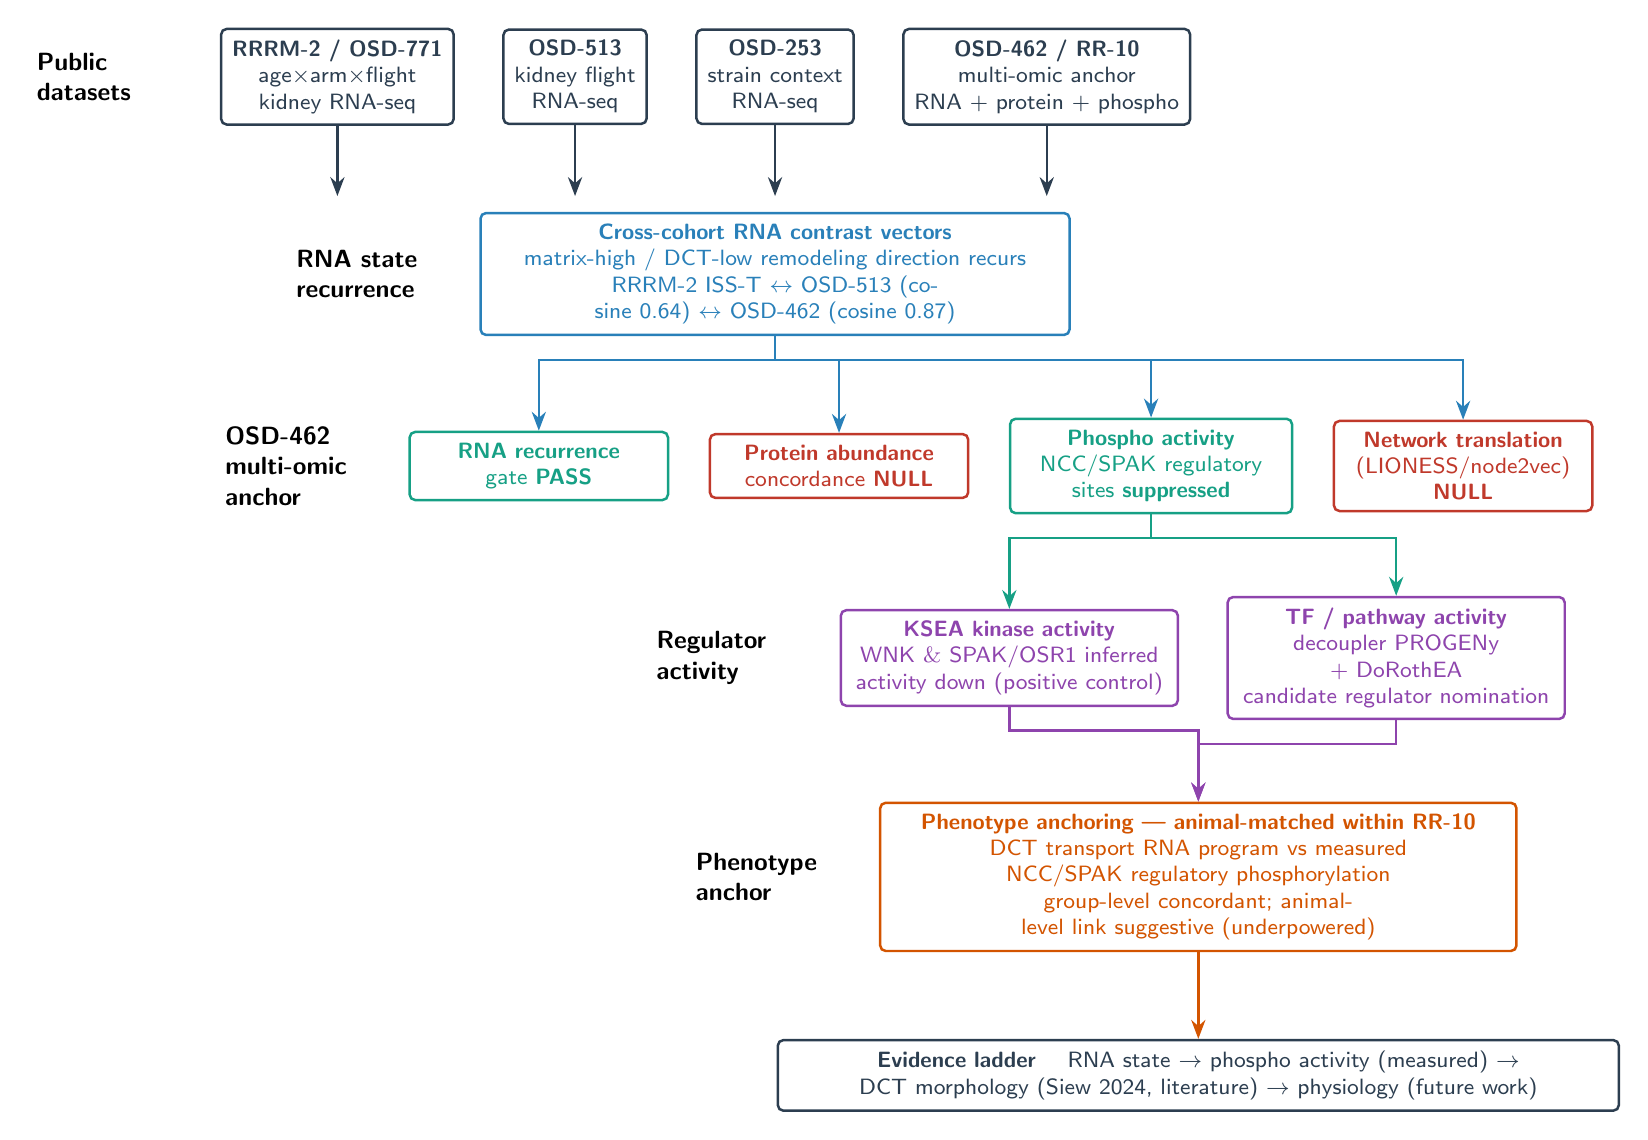
\begin{tikzpicture}[
  font=\footnotesize,
  >={Stealth[length=2.4mm]},
  box/.style={rectangle, rounded corners=2pt, draw=#1, line width=0.9pt,
              text=#1, fill=white, align=center, inner sep=4pt, minimum height=8mm},
  lab/.style={font=\bfseries\small, align=left},
  flow/.style={->, line width=0.9pt, draw=#1},
]

% ---- Row 1: datasets ----
\node[box=cData] (rrrm) {\textbf{RRRM-2 / OSD-771}\\age$\times$arm$\times$flight\\kidney RNA-seq};
\node[box=cData, right=6mm of rrrm] (o513) {\textbf{OSD-513}\\kidney flight\\RNA-seq};
\node[box=cData, right=6mm of o513] (o253) {\textbf{OSD-253}\\strain context\\RNA-seq};
\node[box=cData, right=6mm of o253] (o462) {\textbf{OSD-462 / RR-10}\\multi-omic anchor\\RNA + protein + phospho};
\node[lab, left=4mm of rrrm, text width=18mm] {Public\\datasets};

% ---- Row 2: RNA state ----
\node[box=cRNA, below=11mm of o253, text width=72mm] (rnastate)
  {\textbf{Cross-cohort RNA contrast vectors}\\
   matrix-high / DCT-low remodeling direction recurs\\
   RRRM-2 ISS-T $\leftrightarrow$ OSD-513 (cosine 0.64) $\leftrightarrow$ OSD-462 (cosine 0.87)};
\node[lab, left=4mm of rnastate.west, text width=18mm, anchor=east] {RNA state\\recurrence};

% ---- Row 3: OSD-462 multi-omic anchor (4 boxes) ----
\node[box=cAnchor, below=12mm of rnastate, xshift=-30mm, text width=30mm] (gate)
  {\textbf{RNA recurrence}\\gate \textbf{PASS}};
\node[box=cNull, right=5mm of gate, text width=30mm] (prot)
  {\textbf{Protein abundance}\\concordance \textbf{NULL}};
\node[box=cAnchor, right=5mm of prot, text width=33mm] (phos)
  {\textbf{Phospho activity}\\NCC/SPAK regulatory\\sites \textbf{suppressed}};
\node[box=cNull, right=5mm of phos, text width=30mm] (net)
  {\textbf{Network translation}\\(LIONESS/node2vec) \textbf{NULL}};
\node[lab, left=4mm of gate.west, text width=18mm, anchor=east] {OSD-462\\multi-omic\\anchor};

% ---- Row 4: regulator activity ----
\node[box=cActivity, below=12mm of phos, xshift=-18mm, text width=40mm] (ksea)
  {\textbf{KSEA kinase activity}\\WNK $\&$ SPAK/OSR1 inferred\\activity down (positive control)};
\node[box=cActivity, right=6mm of ksea, text width=40mm] (tf)
  {\textbf{TF / pathway activity}\\decoupler PROGENy + DoRothEA\\candidate regulator nomination};
\node[lab, left=4mm of ksea.west, text width=18mm, anchor=east] {Regulator\\activity};

% ---- Row 5: phenotype anchoring ----
\node[box=cPheno, below=12mm of ksea, xshift=24mm, text width=78mm] (pheno)
  {\textbf{Phenotype anchoring --- animal-matched within RR-10}\\
   DCT transport RNA program vs measured NCC/SPAK regulatory phosphorylation\\
   group-level concordant; animal-level link suggestive (underpowered)};
\node[lab, left=4mm of pheno.west, text width=18mm, anchor=east] {Phenotype\\anchor};

% ---- Row 6: evidence ladder ----
\node[box=cData, below=11mm of pheno, text width=104mm] (ladder)
  {\textbf{Evidence ladder} \quad RNA state $\rightarrow$ phospho activity (measured)
   $\rightarrow$ DCT morphology (Siew 2024, literature) $\rightarrow$ physiology (future work)};

% ---- arrows ----
\foreach \d in {rrrm,o513,o253,o462} \draw[flow=cData] (\d.south) -- ([yshift=2mm]rnastate.north -| \d.south);
\draw[flow=cRNA] (rnastate.south) -- ++(0,-3mm) -| (gate.north);
\draw[flow=cRNA] (rnastate.south) -- ++(0,-3mm) -| (prot.north);
\draw[flow=cRNA] (rnastate.south) -- ++(0,-3mm) -| (phos.north);
\draw[flow=cRNA] (rnastate.south) -- ++(0,-3mm) -| (net.north);
\draw[flow=cAnchor] (phos.south) -- ++(0,-3mm) -| (ksea.north);
\draw[flow=cAnchor] (phos.south) -- ++(0,-3mm) -| (tf.north);
\draw[flow=cActivity] (ksea.south) -- ++(0,-3mm) -| (pheno.north);
\draw[flow=cActivity] (tf.south) -- ++(0,-3mm) -| (pheno.north);
\draw[flow=cPheno] (pheno.south) -- (ladder.north);

\end{tikzpicture}
\end{document}
